\chapter[Analysis]{Analysis}
\label{Chap:Analysis}

This chapter presents a systematic comparative analysis of how the Law and Justice Party functions as a mnemonic warrior across different platforms and media over two electoral cycles. The study draws on a triangulated body of sources, including official party election programs, articles from conservative and liberal news outlets published in both 2015 and 2023, as well as selected social media content. The latter includes posts from the official PiS`s  X account, as well as from prominent party figures, Beata Szydło, Andrzej Duda, Patryk Jaki, Joachim Brudzinski and Mariusz Blaszczak, during the final months of each respective election campaign. Together, these materials provide a multi-layered view of how memory narratives are constructed, circulated, and politicised. The findings of this analysis are organised thematically and will be discussed in the subsequent chapter.

\section{Election Programs}

This section focuses on the official election programs of PiS from 2015 and 2023 as foundational documents for understanding the party's mnemonic strategy. These texts not only outline PiS's political priorities and ideological orientations but also serve as curated expressions of historical memory, national identity, and collective trauma. By comparing these programs, the analysis highlights how PiS uses historical references, victimhood narratives, and cultural symbolism to legitimise its authority and present itself as the guardian of Polish sovereignty and tradition. The comparison reveals both continuity and transformation in the ways PiS deploys memory politics to respond to shifting political landscapes and reinforce its populist-nationalist discourse.

\subsection{Core Values}

Both the 2015 and 2023 election programs of Law and Justice (PiS) emphasise core national values centred on freedom, justice, equality, and the preservation of Polish identity and sovereignty. These values are consistently framed within Poland's historical experiences and cultural heritage, particularly its Catholic tradition and struggles for independence.
Freedom is portrayed not just as individual autonomy but as a communal good rooted in national identity. In the program for the 2015 election, published in 2014, PiS linked freedom to solidarity and community, rejecting the idea that individual liberty opposes collective rights: "\textit{wolność jednostki są związane z solidarnością, która jest podstawą każdej wspólnoty}" ("individual freedoms are linked to solidarity, which is the basis of every community") \citep{pis_program_2014}.

In the 2023 program, freedom is framed as a continuation of Poland's historic struggle for national sovereignty, deeply rooted in national traditions and historical experiences. Independence from foreign influence, especially supranational institutions such as the European Union, is emphasised, as seen in the following passage: "\textit{Jednocześnie sprzeciwiamy się wszelkim próbom odebrania władzy. Narodowi i przekazania jej pozbawionym kontroli instytucjom oraz organizacjom miedzynarodowym}" ("At the same time, we oppose any attempts to take power away from the people and hand it over to unaccountable institutions and international organisations") \citep{pis_program_2023}, which can be understood as Pis opposing all attempts to take power away from the people and handing it over to institutions and international organisations devoid of control.

Justice and equality are presented as moral imperatives and pillars of national order. The 2014 program aligns with Catholic social teaching, citing Pope John Paul II's and Pope Francis's critiques of economic injustice and exclusion \citep{pis_program_2014}. Equality is defined not as uniformity but as respect for individual difference and creative potential: "\textit{Zdajemy sobie sprawę z historycznych obciążeń… na definiowaniu równości}" ("We are aware of the historical burdens... on defining equality) \citep{pis_program_2014}, meaning that the party is aware of the historical burdens that have left their mark on the definition of equality. In 2023, equality is grounded in national dignity and used to critique both past communist hierarchies and post-transition elitism. PiS presents itself as the defender of ordinary citizens against "false elitism" \citep{pis_program_2023}.

The Solidarity movement serves as a central historical reference point. PiS uses it to claim continuity with Poland's moral and patriotic traditions. The 2014 program declares: "\textit{Ruch ten nie mógłby powstać, gdyby nie pontyfikat Jana Pawła II. Nie ma Europy sprawiedliwej bez Polski niepodległej}" ("This movement could not have come into being if it were not for the pontificate of John Paul II. There is no just Europe without an independent Poland") \citep{pis_program_2014}, highlighting the role of Catholic faith in national renewal. PiS positions itself as the guardian of Solidarity's legacy, while accusing its political rivals, particularly PO,  of betraying those ideals and maintaining distorted historical narratives \citep{pis_program_2023}.

The state is depicted not only as a political structure but as a cultural and moral institution essential to democracy and identity. Its legitimacy stems from Poland’s long history of partition and statelessness: "\textit{państwo polskie za wartość najwyższej wagi… podważanie jego suwerenności za niemożliwe do przyjęcia}" ("the Polish state as a value of the highest importance ... undermining its sovereignty as unacceptable") \citep{pis_program_2014}. PiS invokes Catholic social teaching, especially the principle of subsidiarity, to ground its vision of a morally guided state distinct from liberal or technocratic models: "\textit{zasada subsydiarności – dorobek społecznej nauki Kościoła katolickiego}" ("The principle of subsidiarity - the acquis of the social teaching of the Catholic Church") \citep{pis_program_2023}.

Both programs also prioritise family, tradition, and community as vital to national survival. The closing message of the 2015 program affirms: "\textit{Warto być Polakiem. Warto, aby trwały i rozwijały się polskie rodziny... wspólnota wolnych Polaków}" ("It is worth being Polish. It is worth it for Polish families to endure and thrive.... community of free Poles") \citep{pis_program_2014}.

By 2023, PiS presents itself as the moral and political force restoring dignity, justice, and prosperity to the Polish nation. While pledging to reduce social disparities, the party also upholds meritocracy, connecting this stance to Polish traditions of resilience and social mobility. Women's roles are highlighted in the context of traditional values and Catholic heritage, linking historical and contemporary discussions of equality, as emphasised by "\textit{dbać o odpowiednią pozycję kobiet w społeczeństwie}" ("ensure that women have an appropriate position in society") \citep{pis_program_2023}, taking care of the appropriate position of women in society.

In conclusion, both election programs emphasise the importance of upholding core national values. They assert that being Polish and belonging to the Polish national community is worthwhile while maintaining a sovereign, democratic state governed by law \citep{pis_program_2014}. The survival and prosperity of Polish families are declared national priorities. A strong state depends on the nation's development as a community of free individuals, healthy families, a robust economy, and a rich cultural heritage \citep{pis_program_2023}.


\subsection{Othering}

The Law and Justice party frames Polish politics as deeply polarised, dividing the nation into two opposing camps. On the one hand, PiS is positioning itself as the defender of Polish sovereignty, national identity, and traditional values. On the other hand, there is the Civic Platform (PO), closely associated with Donald Tusk and the media elite, whom PiS portrays as representatives of a liberal establishment working against the country's true interestsn \citep{pis_program_2014}. This sharp "us versus them" distinction is central to PiS's political messaging, casting current political struggles as a moral and historical battle over Poland's future.

PiS accuses PO of presenting itself as a force for reform during times of political crisis, only to abandon its promises once in power. After the 2005 elections, PO was seen as publicly endorsing necessary reforms while simultaneously orchestrating a media offensive against the PiS-led government and President Lech Kaczyński. The PO-led government formed in 2007 is described by PiS as a return to pre-2005 governance, dubbed the "Tusk system". Although not composed of former communist elites, this system is framed as equally, if not more, harmful, centralising power, weakening democratic norms, and sustaining structural inequalities \citep{pis_program_2014}.

PiS characterises this system as a "\textit{typowa ekipa restauracji}" ("a typical restoration team"), and warns: "\textit{System ten zagraża zarówno demokracji i prawom obywatelskim jak i wszystkiemu, co decyduje o zdrowym… rozwoju naszej ojczyzny}" ("This system threatens both democracy and civil rights, as well as everything essential to the healthy development of our homeland") \citep{pis_program_2014}.

This portrayal reflects a deeper moral and historical division. PiS presents itself as the rightful heir to the legacy of the Solidarity movement, anti-communist resistance, and Catholic moral values. In contrast, PO is linked to post-communist elites, Western liberal ideologies, and political compromises. By invoking unresolved tensions from Poland's post-1989 transformation, PiS uses this dichotomy to reinforce its legitimacy and cast its opponents as betrayers of national identity and democratic renewal. PiS presents itself as the actual agent of reform, dedicated to meaningful change while confronting resistance from entrenched elites, mainstream media, and the PO-led government. It claims to defend democratic legitimacy, national sovereignty, and the everyday interests of ordinary Polish citizens \citep{pis_program_2014}.

A central battleground in this struggle is the domain of public media and cultural institutions. PiS accuses PO of undermining historical truth and weakening Poland's cultural fabric, citing direct threats to national institutions: "\textit{Trwa atak na Polskie Radio i Telewizję Polską}" ("There is an ongoing attack on Polish Radio and Television") and "\textit{drastycznie zredukowano środki na ochronę zabytków}" ("Funding for the protection of cultural heritage has been drastically reduced") \citep{pis_program_2014}.

In the cultural and memory sphere, PiS portrays PO and its allies as antagonistic to Polish national identity and values. According to PiS, the education system under PO eroded national consciousness and suppressed the teaching of Polish history. Public media are presented as politically and financially undermined, especially in the face of a dominant pro-PO private press. Donald Tusk is directly criticised for weakening public institutions and fostering disorder. Furthermore, PiS argues that scientific and intellectual life under PO suffers from censorship and ideological conformity, posing a threat to academic freedom and open inquiry \citep{pis_program_2014}.

In contrast, PiS presents itself as the protector of national identity, historical memory, and cultural continuity. It promotes public media as a cohesive national force and defends intellectual freedom grounded in Polish traditions. This battle over public values is framed in existential terms: without robust cultural institutions, PiS warns, Poland's historical continuity and national freedom are at risk. As articulated in the 2015 program, memory culture is not just a commemorative practice but the foundation of Polish identity and liberty \citep{pis_program_2014}.

In its foreign policy discourse, PiS contrasts itself with Civic Platform by portraying PO's pro-European stance as compromising Polish sovereignty. PiS presents itself as the defender of national interests, grounded in historical awareness and a strong security posture. It portrays the post-1989 "Third Republic" as a deviation from Poland's historical trajectory, which PiS intends to correct \citep{pis_program_2023}. Opposition parties, especially those aligned with PO, are labelled as liberal and naïve, accused of ignoring the lessons of Polish history, particularly regarding Russian aggression and Western appeasement. The party invokes betrayal narratives, referring to a supposed "German-Russian axis", and criticises foreign policy strategies seen as yielding to supranational pressures. In contrast, figures such as Lech Kaczyński are mythologised as visionary leaders who defended Polish dignity and sovereignty, highlighting a stark divide between PiS and its opponents \citep{pis_program_2023}.

PiS's position on the European Union is cautiously supportive, emphasising the original ideals of integration, solidarity, freedom, and cooperation, while rejecting deeper federalisation. The 2015 program warns against cultural and political homogenisation:

\begin{displayquote}
"\textit{Europa musi pozostać wspólnotą wolności, solidarności i sprawiedliwości, wyrosłą z wielu tradycji narodowych}" ("Europe must remain a community of freedom, solidarity, and justice, rooted in many national traditions") \citep{pis_program_2014}.
\end{displayquote}

While PiS supports EU membership, this is conditional upon the protection of Polish sovereignty, especially regarding national budgets, migration, and cultural identity. The party rejects external "cultural re-education" and pledges to defend the right of each member state to shape its own social and legal order \citep{pis_program_2014}. In the 2023 program, PiS frames EU integration as a national success now threatened by "Brussels-Berlin" dominance and costly policies, such as migration quotas and climate regulations. It contrasts its position with what it calls the opposition's "naïve" embrace of European federalism, which allegedly weakens Poland's autonomy and exposes it to external manipulation \citep{pis_program_2023}.

Ultimately, PiS's foreign policy narrative draws on historical grievances, including the partitions of Poland, to stress the need for self-determination and vigilance in the international arena. The EU is accepted as a framework for cooperation, but only to the extent that it respects the sovereignty, identity, and cultural values of the Polish nation.

Cultural policy in Poland under the Law and Justice party (PiS) has been framed as an ideological battleground essential to the preservation of national identity and historical truth. This has involved a deliberate contrast between PiS and the ruling Civic Platform (PO), which PiS accuses of undermining Polish sovereignty, patriotism, and cultural cohesion \citep{pis_program_2023}. Through cultural institutions, historical narratives, and educational reform, PiS advances a binary framework of "us versus them" to legitimise its vision for Poland's national future.

In the 2015 program, PiS criticised the PO government for allegedly eroding patriotism by prioritising technocratic education over national history, literature, and cultural consciousness. This shift was seen as preventing young Poles from internalising a coherent national identity. State-funded cultural institutions were accused of promoting leftist and anti-patriotic content. Programs designed to support national memory, such as "Patriotism of Tomorrow", were reduced or dismantled, reflecting what PiS viewed as a systemic attack on Polish identity \citep{pis_program_2014}.

The 2010 Smoleńsk plane crash, which claimed the life of President Lech Kaczyński, became a pivotal symbol in PiS's cultural politics. The party claimed that the PO government's handling of the tragedy, including its cooperation with Russia, was suspicious and disrespectful. For PiS, the crash was more than a national trauma; it symbolised the moral and political divide in Poland, casting PiS as the seeker of truth and justice and PO as complicit appeasers \citep{pis_program_2014}. In the election program for 2015, it states: "\textit{Tragedia smoleńska, niezależnie od jej przyczyn, stała się wielkim upokorzeniem państwa polskiego i Polaków... Całkowite oddanie sprawy śledztwa Rosjanom... gra prowadzona w istocie w celu potwierdzenia... wyników rosyjskiego śledztwa}" ("The Smoleńsk  tragedy, whatever its causes, has become a great humiliation for the Polish state and the Polish people.... The total surrender of the investigation to the Russians.... A game played in fact to confirm the ... the results of the Russian investigation") \citep{pis_program_2014},  framing the event as a moment of moral and institutional failure under PO, used by PiS to claim the mantle of truth and justice.

The concept of an existential struggle over memory permeated PiS's cultural narrative. The "them" in this dichotomy, PO, Tusk, and pro-EU elites, were accused of hollowing out state institutions, rewriting history, and acting against national interests. These elites were portrayed as indifferent or hostile to Polish identity, suppressing patriotism in education, media, and science. PiS, on the other hand, styled itself as the true heir to the Solidarity movement and the protector of Polish dignity and sovereignty. For PiS, memory culture was not merely symbolic but foundational to national survival \citep{pis_program_2014}.

Central to the institutionalisation of PiS's historical vision was the role of the Institute of National Remembrance (IPN), which expanded beyond archival and prosecutorial work to serve as a custodian of patriotic memory. The IPN promoted a binary historical narrative: patriots versus enemies, with communists and collaborators vilified \citep{pis_program_2014}.

Funding was allocated to memorialise victims of communist repression, consolidating a collective identity grounded in suffering and resilience. The IPN also assumed control of memorial sites and veteran affairs, creating a centralised apparatus to disseminate a state-sanctioned version of Polish history. PiS reinstated programs like "Patriotism of Tomorrow" to support local historical initiatives and patriotic education, aiming to build a cohesive national consciousness \citep{pis_program_2014}.

By 2023, PiS had further expanded its memory politics through a range of institutions and cultural programs. History was portrayed as a continuous struggle for dignity, independence, and unity, with PiS as the moral custodian of this legacy \citep{pis_program_2023}. Figures such as Józef Piłsudski and Lech Kaczyński were elevated as icons of visionary leadership and national defence \citep{pis_program_2023}. New institutions, including the Polish History Museum, the Pilecki Institute, the Institute of Solidarity Heritage, and the Roman Dmowski \& Paderewski Institute, were established to promote narratives of martyrdom, anti-communist resistance, and Catholic-national values \citep{pis_program_2023}.

Memory was framed as a moral imperative, requiring active stewardship to ensure the nation's resilience and counter historical relativism and liberal interpretations \citep{pis_program_2023}. Educational initiatives, such as "\textit{Poznaj Polskę}" ("Get to know Poland") were utilised to integrate these curated narratives into youth education, promoting patriotic values and historical continuity \citep{pis_program_2023}. Cultural policy thus became a tool to resist perceived foreign influence, safeguard national identity, and position Poland as a leader in regional cultural discourse \citep{pis_program_2023}.

 In conclusion, PiS's approach to cultural policy centres on the instrumentalisation of memory as a political and moral tool. Through an entrenched "us versus them" dichotomy, the party has advanced a vision of national identity rooted in historical martyrdom, traditional values, and resistance to external and internal threats. By institutionalising memory and reshaping cultural discourse, PiS seeks to unify its base while reinforcing its claim to moral authority in Polish public life.


\subsection{Security}

A central theme in Law and Justice's (PiS) 2015 and 2023 election programs is the concept of security, which extends beyond law enforcement or military strength to encompass Polish historical identity and national survival. PiS frames security through collective memory, connecting contemporary policies to Poland's past struggles for sovereignty and civil protection.

For the election in 2015, PiS criticised the Civic Platform (PO) government under Donald Tusk for neglecting public safety and politicising law enforcement, accusing it of fostering a quasi-police state with repression reminiscent of communist-era abuses.

PiS highlighted incidents involving surveillance, retaliation against officials, and suppression of protests, framing these as abuses of state power. The party promised reforms to depoliticise security services, enhance accountability, and restore public trust as a moral and democratic imperative \citep{pis_program_2014}.

By 2023, PiS expanded the security narrative to include existential threats tied to historical experiences of war, occupation, and Soviet domination. Security encompassed military readiness, energy independence, health infrastructure, and cultural-demographic continuity, portraying Poland as a defender of Western civilisation and European values. Historical references legitimised increased defence spending and new laws, such as the Homeland Defence Act, as necessary measures grounded in national memory \citep{pis_program_2023}. The program states:

\begin{displayquote}
    "\textit{Zarówno nasza historia, jak i współczesne wypadki polityczne pokazują nam, że zapewnienie bezpieczeństwa Narodowi stanowi najwyższy obowiązek spoczywający na nas wszystkich. Może być ono rozumiane na wiele sposobów: jako bezpieczeństwo militarne, życia i mienia obywateli, energetyczne, gospodarcze, socjalne czy zdrowotne}" ("Both our history and contemporary political accidents show us that ensuring the security of the Nation is a supreme duty incumbent on all of us. It can be understood in many ways: military security, security of citizens' lives and property, energy security, economic security, social security or health security”) \citep{pis_program_2023}.
\end{displayquote}

In foreign policy, PiS contrasted its assertive stance, emphasising resistance to Russian imperialism, NATO cooperation, and regional initiatives, with PO's alleged passive, clientelist approach. PiS accused the PO of sacrificing Polish sovereignty for EU prestige and dependence on Germany and Russia, blaming it for the failure of Eastern policies \citep{pis_program_2014}.

In conclusion, PiS's approach to security demonstrates its broader mnemonic strategy of embedding political legitimacy in selective historical narratives. By framing security as a moral and existential imperative rooted in Poland's traumatic past, PiS positions itself as the guardian of national survival and sovereign continuity. The linkage between memory and policy enables the party to justify far-reaching actions in law enforcement, military defence, and foreign affairs as acts of historical justice and strategic necessity.


\section{News Articles}

This chapter examines how conservative Polish media outlets narrated the collective memory of the Law and Justice party during two pivotal periods: 2015 and 2023, drawing on publicly accessible articles from platforms such as "\textit{Gazeta Wyborcza}", "\textit{Oko Press}", which tend to be more liberal, and "\textit{Rzeczpospolita}", as well as "\textit{wPolityce}", more conservative news outlets. The analysis focuses on the keyword intersection of "\textit{pamięć}" ("memory") and its variations, as well as PiS, spanning the period from September 1st to October 31st in both 2015 and 2023.  The chapter reveals how historical events, figures, and commemorations are mobilised not only to remember the past but to strategically forge contemporary national identity and legitimise PiS's political project as a mnemonic warrior, one that actively contests and redefines collective memory in Poland's cultural and political landscape.


\subsection{Memory Disputes}

In both 2015 and 2023, conservative media in Poland promoted a memory culture closely aligned with the Law and Justice party, using selective historical narratives to reinforce national identity and political legitimacy. Over the years, memory has been instrumentalised as a tool to cultivate patriotism, moral clarity, and cohesion, thereby embedding collective remembrance into contemporary political discourse.

In 2015, the focus of memory politics centres on patriotism, sacrifice, and resistance against foreign aggression, emphasising religious symbolism and historical clarity. Articles present acts such as the rediscovery and burial of Teofil Jurek as a patriotic and spiritual resurrection \citep{wpolityce_ostatni_2015} and mythologise the Polish countryside as a sacred landscape desecrated by violence.

Wartime imagery and literary references embed emotional patriotism, while the 2015 Russian Duma resolution is framed as aggressive revisionism, opposed by Poland's sovereign memory acts \break\citep{wpolityce_moskiewska_2015}. State commemorations, such as President Duda's visit to the Wujek mine memorial, reinforce PiS's anti-communist legacy. Even protests opposing PiS's judicial reforms are incorporated into memory discourse, reflecting the contested role of memory \citep{wpolityce_prezydent_2015}. Cultural figures like Maria Rodziewiczówna symbolise enduring Polish identity and critique "pseudo-patriotism" \citep{wpolityce_skoro_2015}.

By contrast, 2023's conservative memory politics foregrounds PiS's contemporary political legitimacy and geopolitical strategy. Memory is deployed to validate current governance, especially around Prime Minister Morawiecki's exposé and no-confidence vote, where achievements are framed as continuations of a successful Polish past and opposition narratives are delegitimised \citep{wpolityce_relacja_2023}. Additionally, the memory of Polish-Ukrainian historical ties is instrumentalised to strengthen Poland's role in regional alliances and resistance against Russian aggression, highlighting shared heritage and moral solidarity \citep{wpolityce_wszystkie_2023}. This reflects a shift from primarily commemorative narratives toward strategic uses of memory for political consolidation and international positioning.

In 2015, liberal media framed the parliamentary elections as a process of political and social othering, where PiS excluded and delegitimised opposition groups to solidify its dominance. Opposition parties and institutions like the Constitutional Tribunal were cast as alien or hostile to the "true" Polish identity, undermining their legitimacy and marginalising dissenting voices within the national discourse \citep{wronski_pis_2015}. This othering was seen as a deliberate strategy to consolidate power by fostering division and portraying opposition actors as threats to the nation.

By 2023, liberal media critique of PiS's use of memory had deepened and expanded, focusing on the party's systematic instrumentalisation of history across multiple domains, including education, public institutions, political campaigns, and commemorative practices. The politicisation of education, exemplified by figures like Roman Kowalczyk, who promoted nationalist memory and pro-government narratives in schools, exemplifies attempts to shape collective memory and suppress pluralism \citep{kowalczyk_pis-owska_2023}.

Similarly, the dismantling of meritocratic and independent scientific institutions such as the National Science Centre under Minister Przemysław Czarnek is presented as an attack on institutional memory and professional standards \citep{blocki_byly_2023}.

In public spaces, projects like the "Lech Kaczyński Centre for Truth and Reconciliation" in Chełm are criticised as undemocratic impositions prioritising symbolic memory over community needs \citep{brzuszkiewicz_w_2023}. Broader political manoeuvres, including the politicisation of the Constitutional Tribunal, the use of controversial court rulings, and surveillance via Pegasus, are depicted as efforts to embed conservative ideology within public consciousness and suppress alternative narratives \citep{izdebski_nierowne_2023}.

Liberal commentators advocate for a memory culture rooted in inclusivity, peace, and democratic values, cautioning against mythologising sacrifice and conflict without tangible progress \citep{liliental_przerazmnie_2023}. Overall, the 2023 liberal critique portrays PiS as intensifying its control over collective memory to maintain political power, distort democratic dialogue, and limit the diversity of historical understanding. Furthermore, Jarosław Kaczyński´s growing importance in decision-making for the party´s vision is highlighted \citep{okopress2023lists}. 

While the 2015 liberal media highlighted political othering as a divisive strategy, the 2023 reporting covers a more institutionalised manipulation of memory that permeates education, science, public space, and governance.


\subsection{Smoleńsk and Solidarność}

The instrumentalisation of memory surrounding the Smoleńsk tragedy and Solidarność plays a central role in the political narratives constructed by PiS and is portrayed distinctly in conservative and liberal Polish media. These portrayals reveal contrasting perspectives on how PiS uses historical memory to consolidate power, shape national identity, and influence public discourse.

In 2015, conservative media emphasised the moral and cultural significance of Solidarność as a faith-based and uniquely Polish movement deeply intertwined with Catholic values. An article highlighted Solidarność’s "\textit{głęboką wiarą w Pana Boga i wartościami konserwatywnymi, to absolutny ewenement na skalę światową}" ("deep faith in the Lord God and conservative values, is an absolute rarity on a global scale") \citep{wpolityce_solidarnosc_2015} as "an absolute global phenomenon" that stood apart from secular labour movements elsewhere \citep{wpolityce_solidarnosc_2015}. This religious and patriotic framing extended to the Smoleńsk plane crash, portrayed as a profound national trauma obscured by political deception and official neglect.

The poetry anthology "Antologia Smoleńska", described as "a clear and courageous voice from the Polish literary community in defence of truth", symbolised cultural resistance and a demand for justice \citep{wpolityce_antologia_2015}. Conservative commentators criticised the presence of communist monuments, such as the memorial Czynu Rewolucyjnego in Rzeszów, labelling it a "criminal symbol" while lamenting the lack of a proper memorial for the Smoleńsk victims \citep{wpolityce_historyk_2015}.

Political figures affiliated with PiS emphasised the significance of Lech Kaczyński's memory as central to national revival and moral renewal \citep{wpolityce_profesor_2015}. President-Elect Andrzej Duda called Kaczyński’s mission: "\textit{kontynuacja jego dzieła jest dla nas patriotycznym i ludzkim zobowiązaniem}" ("continuing His work is a patriotic and human obligation for us") \citep{wpolityce_lech_2015}. At the same time, Jarosław Kaczyński framed the struggle for memory as a battle for "truth and dignity" against an "industry of contempt" \citep{wpolityce_lech_2015}. Jarosław Kaczyński's speeches at the Marsz Pamięci condemned the "triumph of lies and injustice" \citep{wpolityce_kaczynski_2015}, linking this moral decay to the failure to honour Smoleńsk victims and calling for a national spiritual rebirth \citep{wpolityce_kaczynski_2015-1}.

In conservative discourse around 2023, PiS's use of Smoleńsk and Solidarność continued to symbolise national martyrdom and resistance against foreign and internal enemies. General Lech Majewski's controversial role after Smoleńsk was criticised for shifting blame away from Russian air traffic control to Polish pilots, reflecting alleged pro-Russian sympathies within parts of the military establishment \citep{wpolityce_strzezcie_2023}. Conservative media framed the annual "\textit{miesięcznice commemorations}" as sacred rituals affirming Polish unity, contrasting sharply with opposition figures like Radosław Sikorski, whose critical remarks were portrayed as disrespectful provocations undermining national solidarity \citep{wpolityce_sikorski_2023}. This narrative positions PiS as the defender of Polish dignity and historical truth by mobilising collective memory around themes of victimhood and patriotism.

Liberal media, by contrast, critiqued PiS's selective and instrumental use of the Smoleńsk tragedy and Solidarność as divisive and manipulative. PiS was accused of deepening political polarisation and undermining democratic discourse by promoting a narrative that excludes rival figures such as Lech Wałęsa. For example, during the 2015 commemoration of Lech Kaczyński's presidential oath, the refusal to honour Wałęsa alongside Kaczyński was seen as an intentional shaping of memory to serve political ends. Jarosław Kaczyński's comment that honouring Wałęsa was "\textit{cokolwiek bezprzedmiotowe}" ("anything but pointless") \citep{gazeta_wyborcza_sejm_2015} exemplifies this deliberate exclusion.

The party's promotion of the assassination theory regarding the 2010 crash reinforced narratives of martyrdom and betrayal, with Jarosław Kaczyński denouncing the dissolution of the Smoleńsk subcommission as a "solemn gift to Putin" \citep{czuchnowski_koniec_2023}.

Liberal commentators warned that this exploitation of national trauma creates a "Smoleńsk religion" that fuels ideological "fumes" and poisons public debate, as noted by Paweł Adamowicz \citep{sandecki_adamowicz_2023}. The conflict between Jarosław Kaczyński and Lech Wałęsa, including Wałęsa's defamation lawsuit and its subsequent challenge at the European Court of Human Rights, highlights ongoing tensions between the control of political narratives and freedom of expression \citep{woznicki_kaczynski_2023}. Additionally, the Civic Platform's attempt in 2015 to include Wałęsa in official commemorations was rejected by PiS, which was accused of manipulating historical memory to divide, rather than to unite Poles \citep{gazeta_wyborcza_pis_2015}.

In conclusion, conservative media portray PiS's instrumentalisation of Solidarność and the Smoleńsk tragedy as a moral and patriotic project rooted in faith, martyrdom, and national unity. This use of memory serves to legitimise the party's political agenda and frame it as the defender of Polish dignity and historical truth. Liberal media, however, interpret the same phenomena as divisive strategies that manipulate history to deepen polarisation and undermine democratic pluralism. These divergent portrayals underscore the contested nature of collective memory in Poland and its ongoing significance in political struggles.

\subsection{Catholicism}

This analysis explores how conservative and liberal Polish media portray PiS's instrumentalisation of Catholicism, focusing on the party's use of the Church's image and legacy to advance its political goals. Both conservative and liberal perspectives recognise Catholicism's central role in Polish identity and politics. Yet, they differ sharply in their interpretation of PiS's relationship with the Church and the consequences of this alliance.

Conservative media depict PiS as the legitimate defender of Catholic values and the legacy of Pope John Paul II, presenting the party’s actions as faithful to Church teachings and aligned with national interests. PiS is portrayed as safeguarding Poland: "\textit{Pis wykreował się na strażnika wartości katolickich i spuścizny Jana Pawła II, przeciwstawiając się lewicowym atakom wymierzonym w tożsamość i dziedzictwo chrześcijańskie}" ("\textit{Continuing his work is a patriotic and human obligation for us}") \citep{szuldrzynski_michal_2023}.

The party's opposition to EU migration policies is framed as consistent with protecting "the Church's moral order and the nation's cultural integrity", symbolised by Prime Minister Mateusz Morawiecki's invocation of John Paul II's motto "Do not be afraid!" \citep{szuldrzynski_michal_2023}. Conservative media also accused political opponents of hypocrisy, suggesting that critics misuse John Paul II's name to promote agendas contrary to Church teaching, thereby positioning PiS as the "proper custodian of Catholic values" that stands against secularisation \citep{szuldrzynski_michal_2023}. Although acknowledging controversies such as clerical abuse scandals, conservative outlets dismiss them as politically motivated attacks designed to weaken Poland's spiritual foundation, equating the defence of John Paul II's legacy with the defence of the nation itself \citep{kolanko_kampania_2023}.

In contrast, liberal media portray PiS's relationship with Catholicism as a strategic political exploitation aimed at consolidating power by mythologising history and sanctifying religious identity. The party is criticised for promoting "national amnesia" and "historical whitewashing" \citep{mrozek_jak_2023}, particularly by sanitising John Paul II's image to appeal emotionally to conservative voters while suppressing more complex truths, such as Poland's wartime involvement in anti-Jewish violence \citep{mrozek_jak_2023}. The liberal perspective highlights PiS's aggressive defence of John Paul II amid sexual abuse allegations, dismissing critics as "enemies of Polish dignity" and polarising society between older, devout voters and younger Poles rejecting Church authority \citep{gadomski_awantura_2023}. Parliamentary theatrics, including "shouting down opposition and wielding portraits" \citep{wronski_sejm_2023}, are seen as attempts to weaponise collective memory and silence dissent, deepening social divisions by framing opposition as threats to sacred national values \citep{wronski_sejm_2023}.

PiS's conflation of faith and nationalism is underscored by Jarosław Kaczyński's claims that the current government undermines Catholic rights in favour of "leftist ideologies," revealing deliberate instrumentalisation of religion to mobilise the conservative base and marginalise pluralism \citep{kondzinska_pis_2023}. Stefan Chwin further critiques PiS for politicising Catholicism as a tool to "silence dissent and define national identity," warning that this strategy alienates younger generations and risks accelerating the decline of the Church's credibility in Poland \citep{chwin_stefan_2023}.

Both conservative and liberal media agree that PiS utilises Catholicism to bolster its political legitimacy and shape Polish identity. However, conservatives frame this alliance positively, emphasising protection of tradition, moral clarity, and national unity. Liberals, by contrast, view PiS's use of Catholicism as manipulative and divisive, fostering social polarisation, historical distortion, and democratic backsliding.

\pagebreak

In conclusion, the portrayal of PiS's instrumentalisation of Catholicism reveals deep divisions in Polish media and society. Conservative outlets celebrate the party as the proper guardian of faith and nation, while liberal voices warn against the dangers of politicising religion to suppress dissent and rewrite history. These contrasting narratives reflect broader conflicts over memory, identity, and power in contemporary Poland.

\subsection{Holocaust}

This analysis compares conservative and liberal media portrayals of the ruling Law and Justice party's instrumentalisation of Holocaust memory in Polish political discourse. Both perspectives acknowledge the use of Holocaust symbolism by PiS but differ sharply in their evaluation of its appropriateness and consequences.

Conservative media present PiS's use of Holocaust memory as a justified defence of national dignity against offensive and disrespectful attacks. In response to journalist Tomasz Lis' provocative tweet referencing Nazi gas chambers, PiS released a campaign video invoking Auschwitz imagery to condemn opposition marches, framing the party as protecting the memory of Holocaust victims from insult \citep{wpolityce_pis_2023}. Conservative outlets defended this as a necessary reaction, accusing critics and institutions like the Auschwitz Museum of hypocrisy and selective outrage.

For example, Member of the European Parliament (MEP) Tomasz Poręba argued that "critics were silent" when Lis' tweet first appeared but only objected after PiS responded, highlighting double standards in the political use of Holocaust memory \citep{wpolityce_pis_2023}. Additionally, conservative commentary criticised the Auschwitz Museum for condemning PiS's campaign while remaining silent when PiS itself was compared to Nazis by opposition figures, asserting that "genuinely protecting the memory of Auschwitz victims requires impartiality, not selective outrage" \citep{wpolityce_gdy_2023}. This framing positions PiS as a moral guardian who defends national trauma from misuse and political attacks.

Liberal media, in contrast, condemn PiS's use of Holocaust imagery as an unethical political weaponisation that degrades national symbols and poisons public discourse. They highlight the 2023 campaign spot employing harrowing visuals from Auschwitz to link opposition protests to disrespect for Holocaust victims and Polish history, describing it as crossing "an ethical boundary" and provoking condemnation from the Auschwitz Museum as "an insult to victims" \citep{kondzinska_spot_2023}. Liberal commentators view this as part of a broader PiS pattern, where traumatic memories of World War II and the Holocaust are exploited for electoral advantage, including "justifying anti-refugee policies" and politicising commemorations such as the Warsaw Ghetto Uprising \citep{wielinski_pis_2023}.

The symbolic importance of Auschwitz as a universal warning against hatred is said to be undermined by PiS's divisive tactics, risking "moral degradation of national symbols" and threatening democratic debate \citep{kondzinska_spot_2023}. Moreover, liberal media criticised the portrayal of politicians Mariusz Kamiński and Maciej Wąsik as concentration camp prisoners by PiS supporters, denouncing it as a "\textit{ypaczenie prawdy historycznej i trywializowanie cierpienia ofiar Holokaustu}" ("distortion of historical truth and a trivialisation of the suffering of Holocaust victims"), which reflects "dangerous moral degradation in political discourse" \citep{wantuch_przy_2023}.

Both media perspectives acknowledge that Holocaust memory is a powerful and contested element in Polish politics. However, conservatives view PiS's actions as protective and justified, while liberals see them as manipulative and damaging. Conservatives emphasise accusations of hypocrisy against PiS's critics and call for impartiality in safeguarding Holocaust memory, whereas liberals stress the moral and democratic costs of politicising such trauma.

In conclusion, the portrayals reflect deep divisions in how Holocaust memory is mobilised in Poland's political culture. Conservative media frame PiS's instrumentalisation of Holocaust history as a defence of national honour and moral seriousness, while liberal media warn against its exploitation for partisan gain that degrades collective memory and democratic values. This contrast highlights the sensitive and polarising nature of Holocaust remembrance in contemporary Polish political discourse.

\section{Social Media}
\label{sec:social_media}

This subsection examines the use of social media by key actors of the Law and Justice party during two electoral periods. The analysis focuses on activity on X (formerly Twitter) between September 1st and October 31st in both years, thereby capturing the final phase of campaigning in the run-up to the parliamentary elections on October 25th, 2015, and October 15th, 2023.

The dataset includes tweets by PiS's official account, as well as those of prominent party figures, including Beata Szydło, Andrzej Duda, Patryk Jaki, Mariusz Błaszczak, and Joachim Brudziński. 

\pagebreak

While Jarosław Kaczyński and Mateusz Morawiecki were central political actors during the period under study, they are not included in the dataset because Kaczyński only joined the platform in 2024 and Morawiecki in 2017.

In total, the corpus comprises 2,332 tweets from 2015 and 2,455 tweets from 2023, amounting to approximately 100 MB of text data \citep{rybicki_2025_16933320}. These datasets provide the empirical foundation for the following analysis of how PiS and its representatives addressed questions of populism, illiberalism, and memory culture across two distinct electoral cycles.

A comparison of posting behaviour across the two campaigns reveals significant temporal differences. In 2015, activity levels on election day itself peaked, whereas in 2023 output dropped almost completely. Histograms of posting frequency further show that the official PiS account remained the most active actor across both election cycles, outpacing individual politicians.

\begin{figure}[h!]
\centering
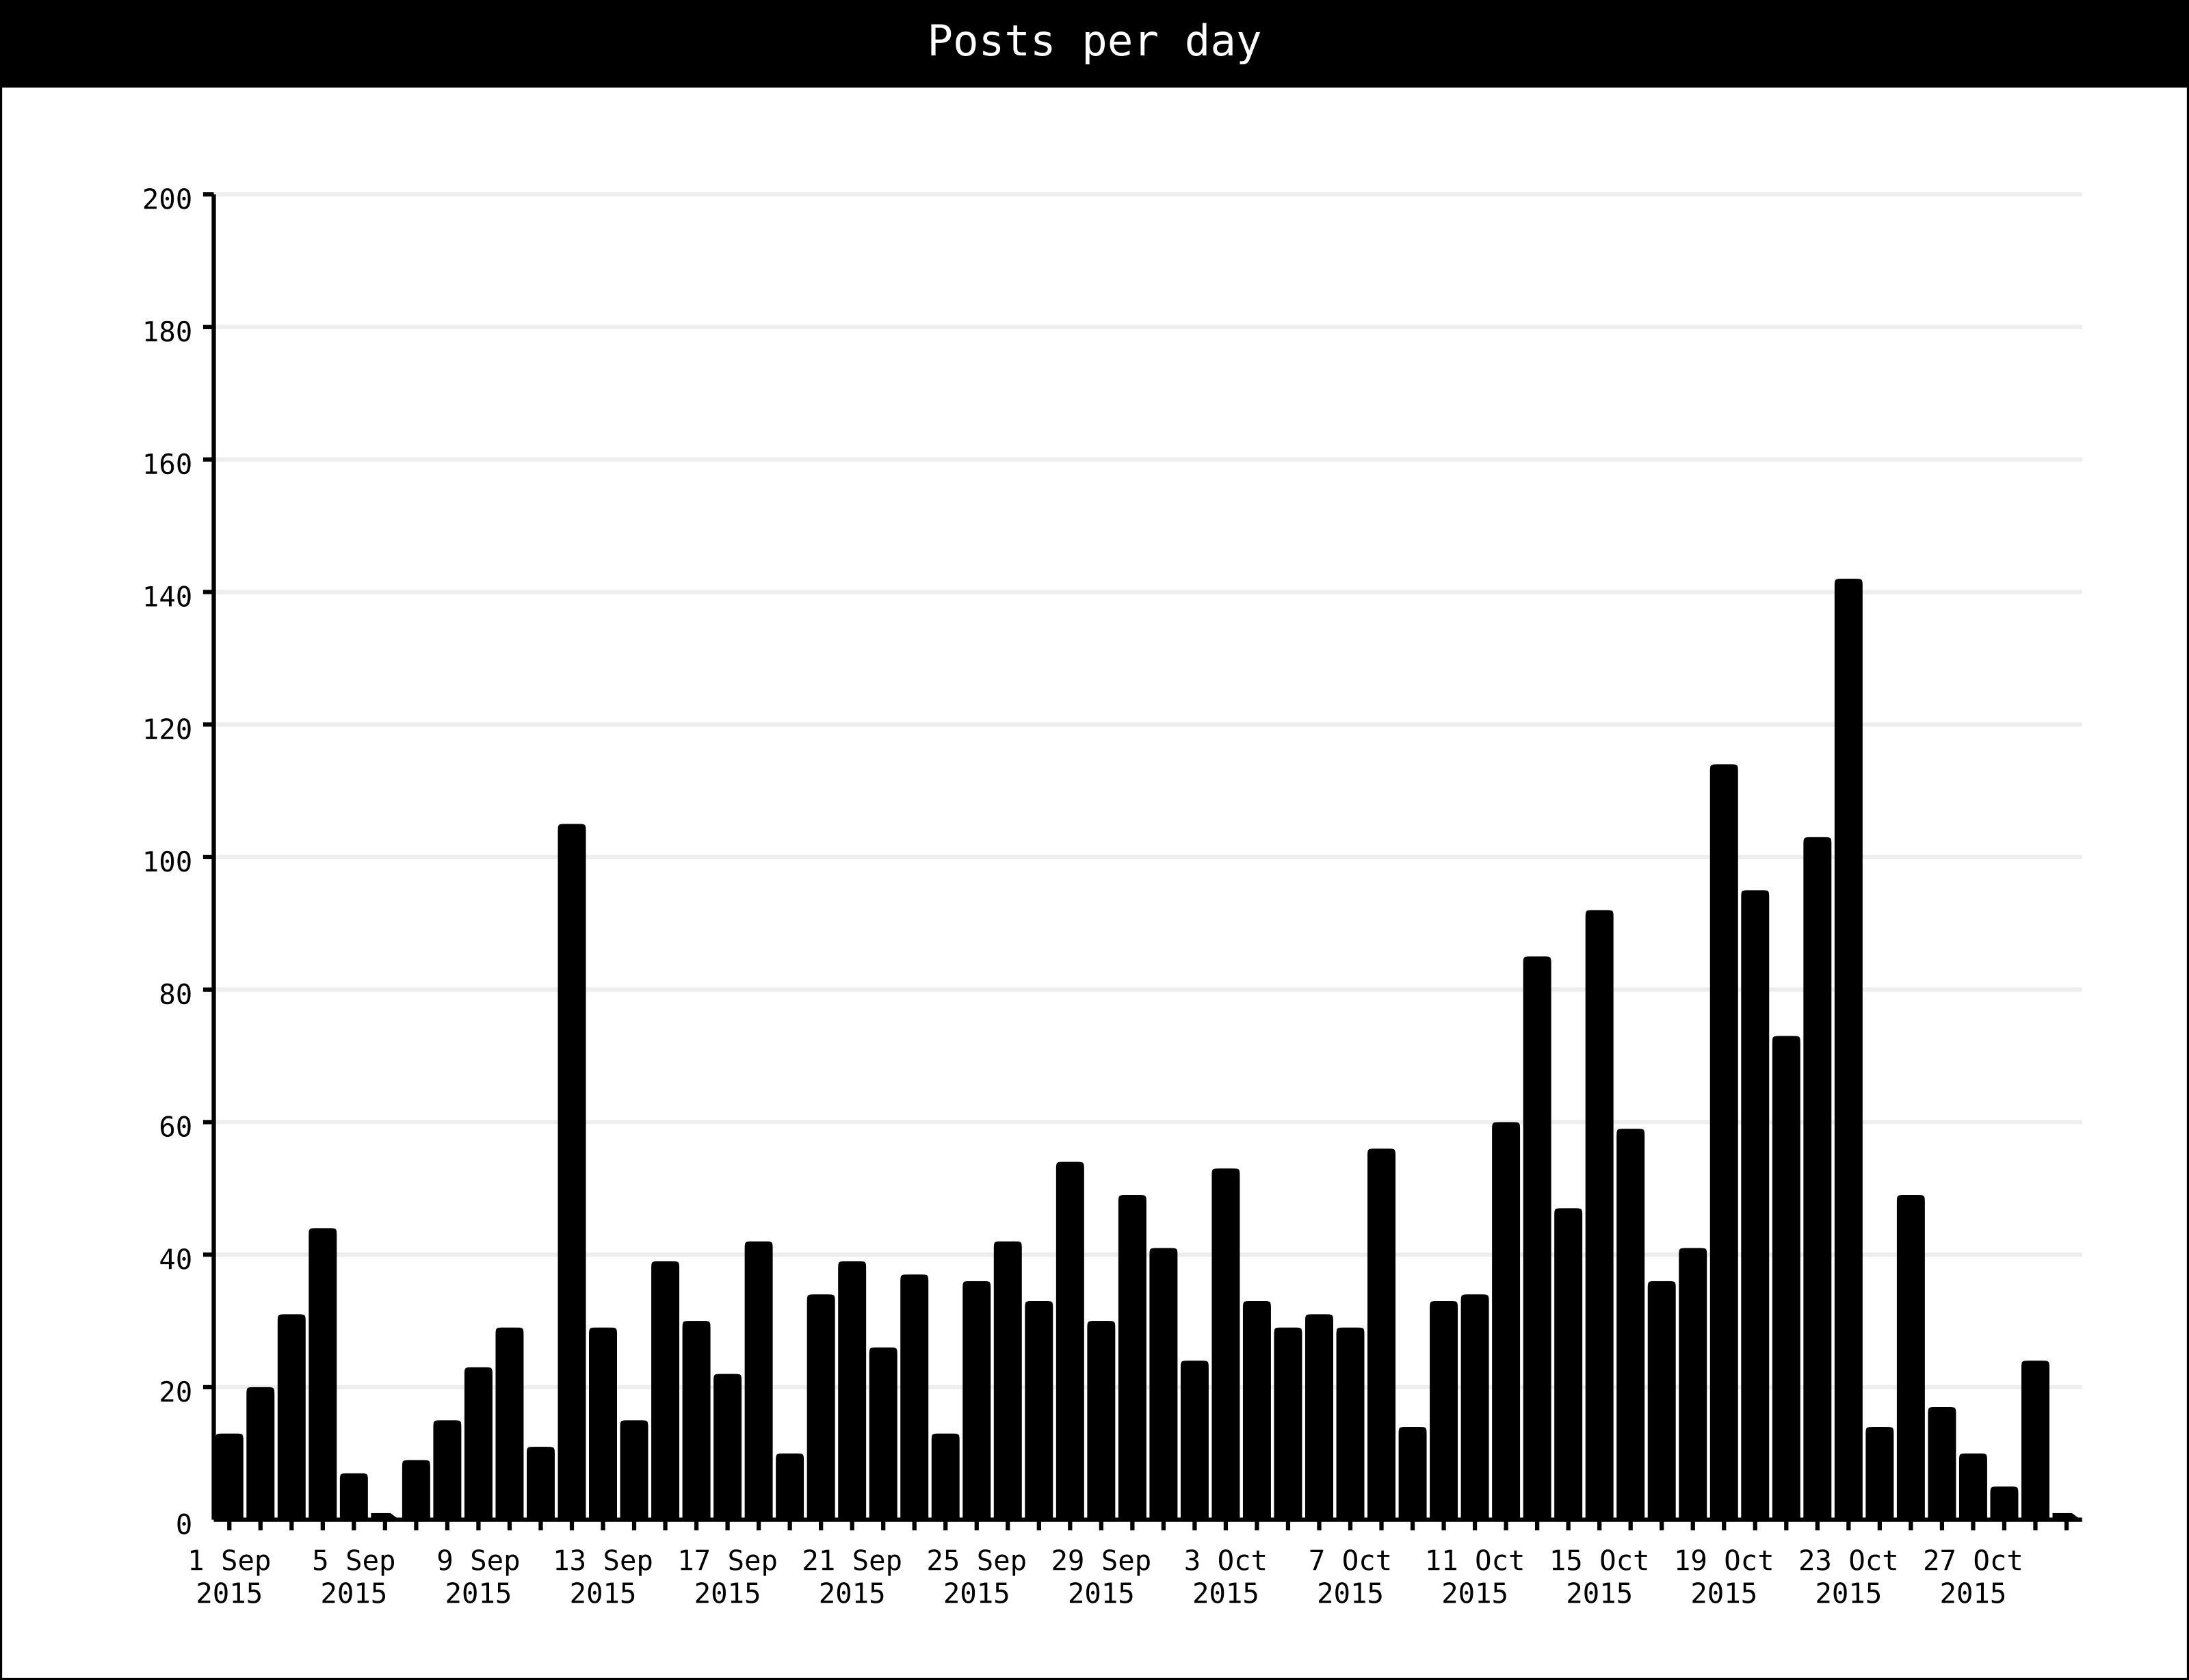
\includegraphics[width=\linewidth]{Graphics/histogram-2015.png}
\caption{Post Histogram (2015)}
\end{figure}

\pagebreak

The histogram displays the daily posts from all monitored accounts from September 1st to October 31st, 2015. Posting was modest through early September, typically below 40 per day, with a single outlier around September 12 at roughly 100 posts. From late September into October, the series rises steadily, with frequent surges in the 60-100 range. 

Activity peaks in the final campaign week (around October 19-24) at approximately 140–145 posts per day, before dropping back toward lower levels at the end of the month \citep{rybicki_2025_16933320}.

\begin{figure}[h!]
\centering
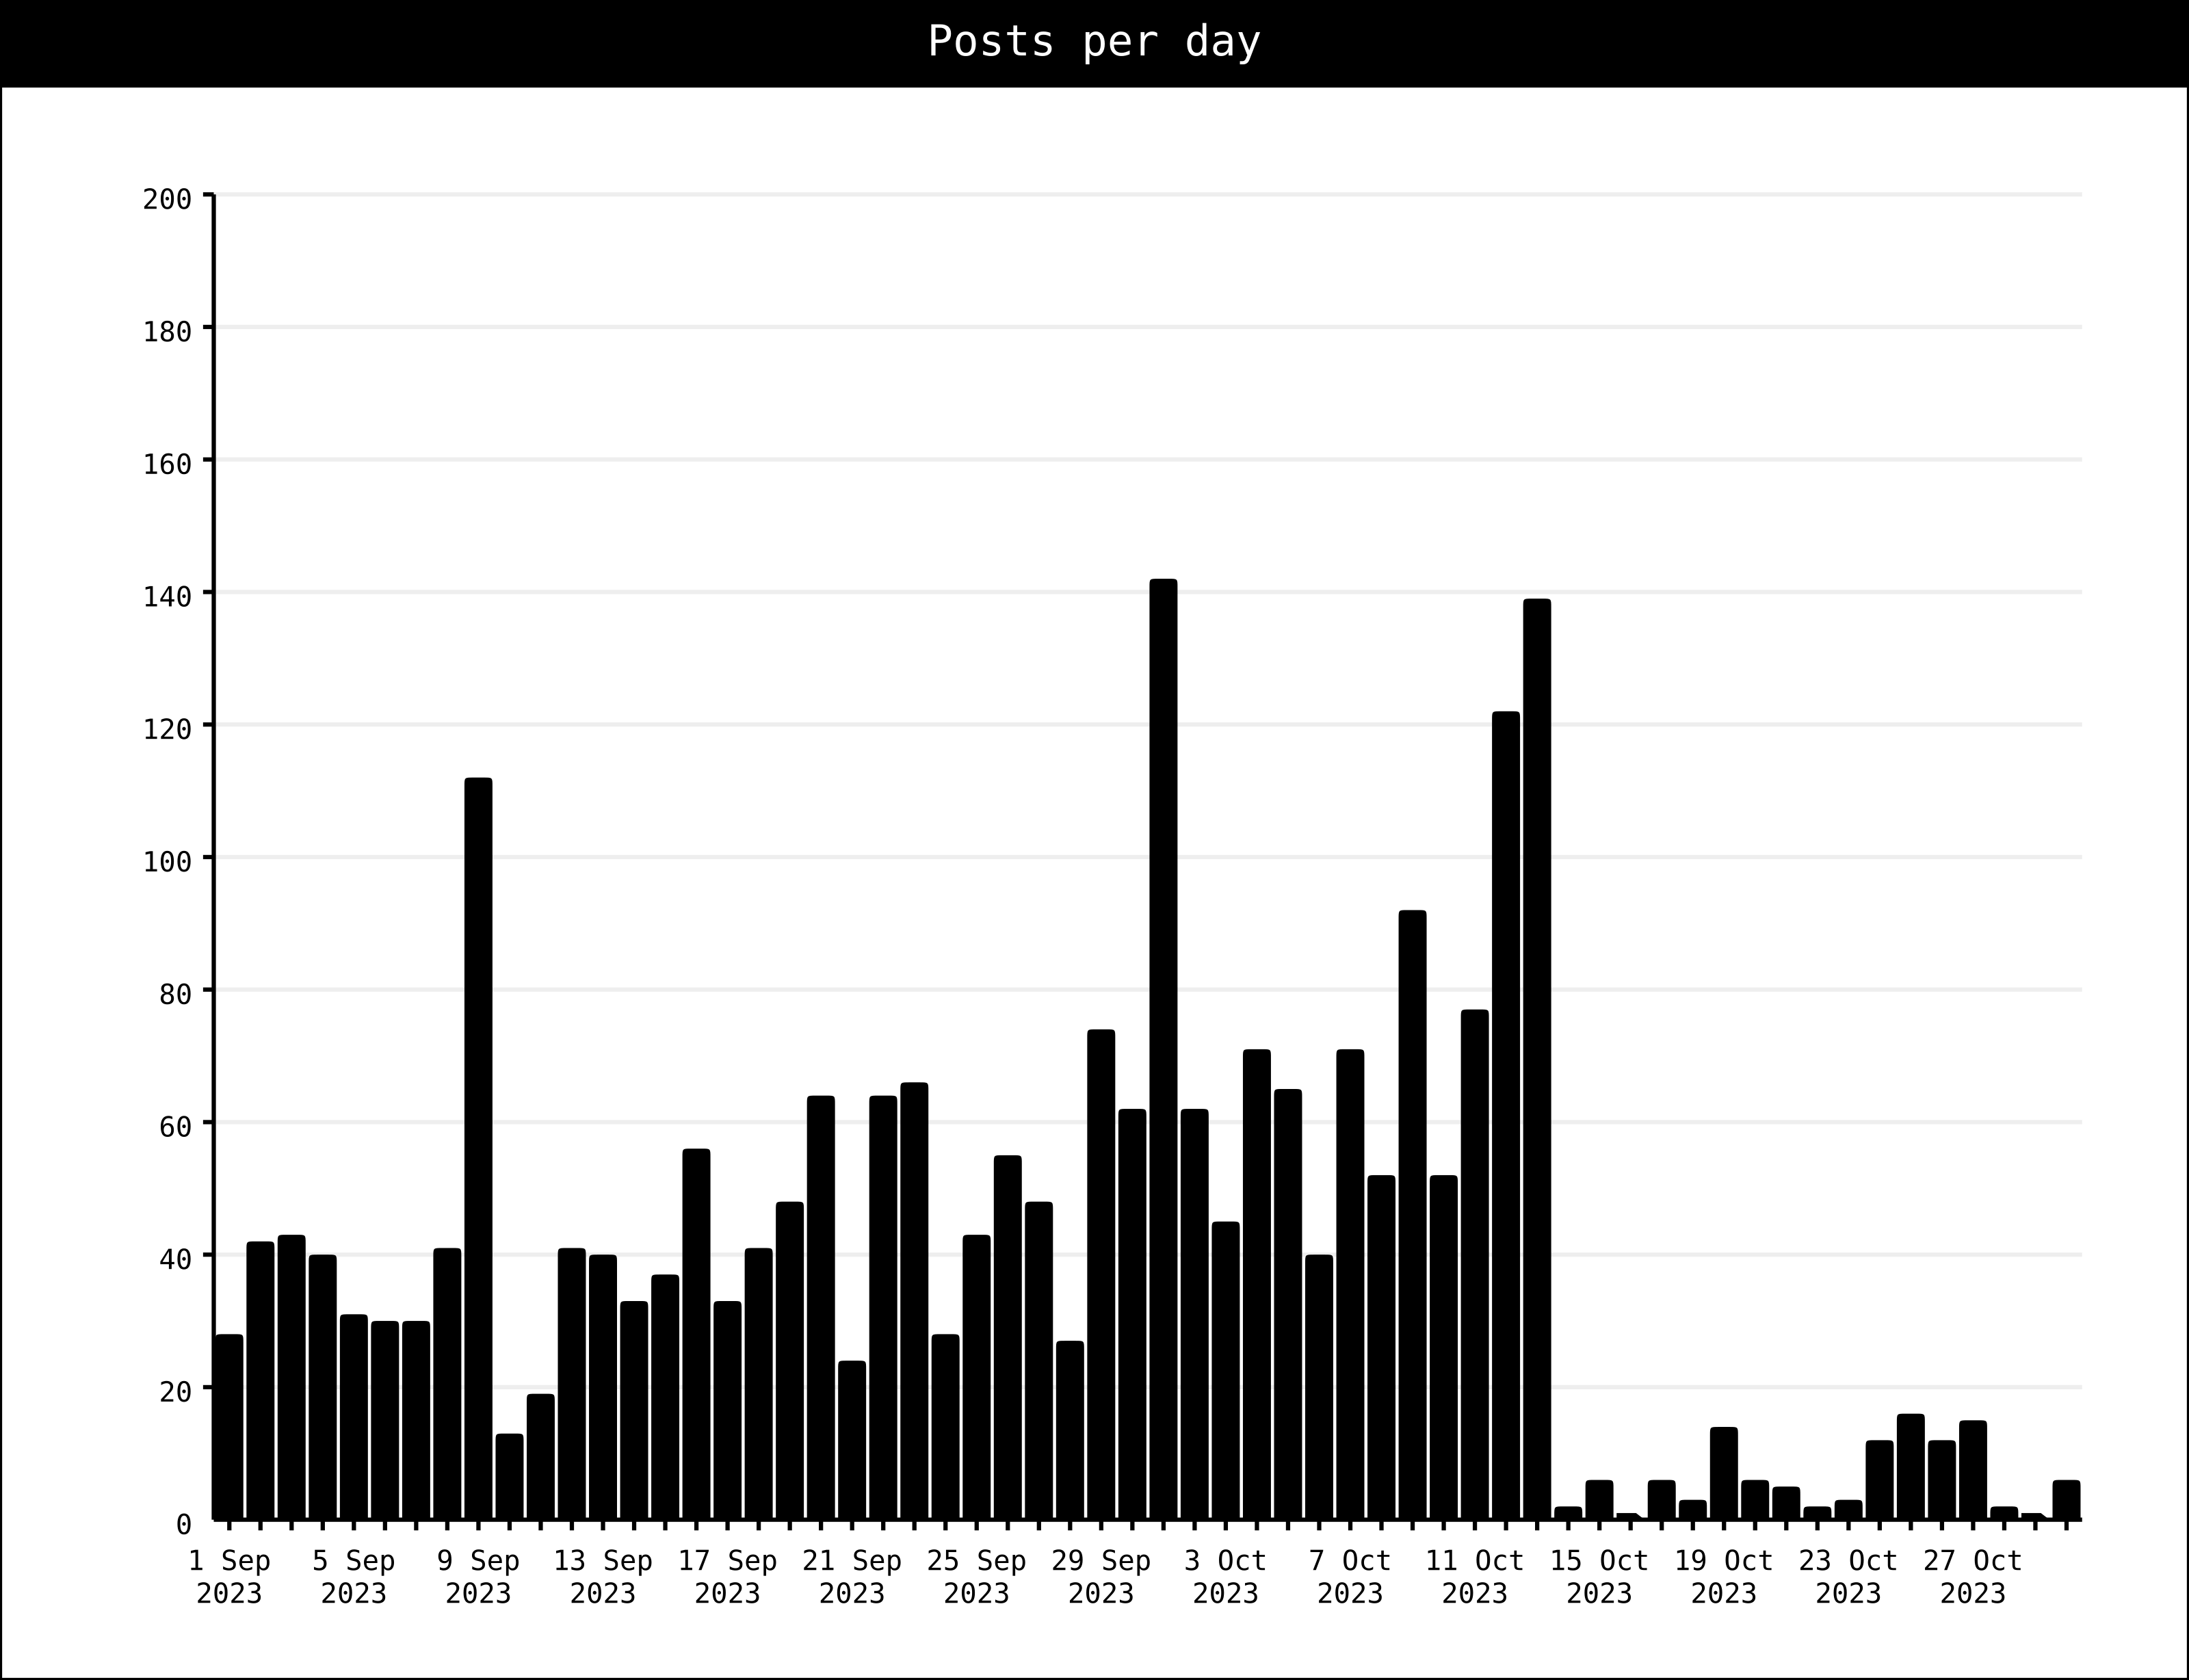
\includegraphics[width=\linewidth]{Graphics/histogram-2023.png}
\caption{Post Histogram (2023)}
\end{figure}

The histogram plots daily posts by all monitored accounts from September 1st to October 31st 2023. Activity in early September is moderate, typically between 25 and 50 posts per day, with an early spike around September 9 exceeding 110. Posting intensifies toward late September and the first half of October, with repeated surges above 70–120 and prominent peaks around late September and October 15 approaching 140 posts per day. After mid-October, the volume collapses to single digits, with only occasional small bumps below 20 through the end of the month \citep{rybicki_2025_16933320}.

\subsection{Othering}

In terms of content, a consistent feature of PiS communication since 2015 has been the construction of external and internal enemies. Russia, Germany, and the European Union emerge as recurrent foes, often linked together in a single narrative. Already during the 2015 campaign, Beata Szydło opposed the idea of a political "reset" with Russia, framing such a position as a dangerous concession by the Civic Platform (PO) government \citep{pisorgpl2015a}. In the 2023 campaign, this rhetoric was intensified and broadened, with PiS representatives repeatedly accusing PO and Donald Tusk of subordinating Poland to German and Russian interests \citep{pisorgpl2023a}. Similarly, Defence Minister Mariusz Błaszczak accused the opposition of risking national security by supposedly preparing to cede half the country to Russia \citep{pisorgpl2023b}.

Such claims often fused historical memory, sovereignty, and security concerns. For example, PiS leaders described Poland under PO–PSL rule as a "German Russian condominium," while also charging the opposition with endangering Poland's territorial integrity by allegedly considering territorial concessions to Russia \citep{pisorgpl2023c}. Furthermore, relations with neighbouring states, such as Ukraine, Lithuania, and members of the Visegrád Group, were also reframed through this lens, with PiS portraying the opposition as weakening regional alliances to the benefit of Germany and Russia \citep{pisorgpl2023d}.

Other PiS representatives further sharpened these accusations. MP Radosław Fogiel directly linked the PO government’s Russia policy to both Moscow and Berlin, emphasising German praise for Donald Tusk after the Smoleńsk disaster: 

\begin{displayquote}
    "\textit{Rząd D. Tuska prowadził wobec Rosji politykę resetu… B. Komorowski spotykał się wtedy z kanclerz Niemiec A. Merkel, która kierowała pochwały wobec D. Tuska…}" ("D. Tusk's government pursued a policy of reset towards Russia… B. Komorowski met with German Chancellor A. Merkel, who praised D. Tusk…") \citep{pisorgpl2023c}.
\end{displayquote}

\pagebreak

Prime Minister Mateusz Morawiecki complemented this narrative by embedding it in a broader populist discourse, contrasting PiS’s defence of "normality" with the alleged corruption of the opposition: 

\begin{displayquote}
    "\textit{Chcemy, aby w Polsce było normalnie - tymczasem dla Platformy normalność to obrona elit. Pieniądze szybciej uciekały z budżetu za rządów PO-PSL niż Tusk uciekł do Brukseli"} ("We want things to be normal in Poland — meanwhile, for the Platform, normality means defending the elites. Money drained from the budget faster under PO-PSL rule than Tusk fled to Brussels") \citep{pisorgpl2023d}.
\end{displayquote}

This continuity between 2015 and 2023 underscores the centrality of enemy construction in PiS's political communication. The tendency to link domestic rivals with external adversaries not only serves populist mobilisation but also anchors current conflicts in a longer historical narrative of betrayal and dependence. Across both campaigns, PiS's strategy thus reveals a striking continuity of rhetorical enemy construction, combining accusations of betrayal, foreign subordination, and the defence of corrupt elites.

PiS campaigns systematically frame Tusk and PO as political enemies, with a noticeable escalation in the number of attacks between 2015 and 2023. In 2015, party officials emphasised their confidence and dismissal of the opposition, portraying PO as non-threatening \citep{pisorgpl2015b}. In 2015, PiS politicians emphasised confidence against the opposition, with Stanisław Karczewski highlighting Beata Szydło's debate performance and declaring that the party was not afraid of PO \citep{pisorgpl2015b}. \\

\vspace{1cm}

\begin{table}[H]
    \centering
    \begin{tabular}{p{4cm}p{4cm}p{4cm}}
        \toprule
        \textbf{Phrase} & \textbf{Amount of posts 2015}  & \textbf{Amount of posts 2023} \\ \midrule
        Tusk & 1 & 220  \\
        PO & 79 & 201  \\ \bottomrule
    \end{tabular}
    \caption{Usage of "PO" and "Tusk" on Twitter/X \citep{rybicki_2025_16933320}}
    \label{tab:phrases-comp-2015-2023}
\end{table}

PiS campaigns consistently construct Donald Tusk and PO as political enemies, with a sharp increase in attack volume from 2015 to 2023. By 2023, the rhetoric had intensified. Jacek Brudziński criticised recycled opposition narratives and denounced them as "pathetic and hateful", emphasising PiS's moral and political superiority \citep{jbrudzinski2023}.

Minister of Defence Mariusz Błaszczak directly framed PiS as the guarantor of national security while blaming PO-PSL for endangering the country. He emphasised:

\begin{displayquote}
    "\textit{Zasługujemy na to, aby żyć w bezpiecznej Polsce! … To rząd PO-PSL likwidował jednostki wojskowe i narażał nas na straszne niebezpieczeństwo… Tylko wolna i suwerenna Polska jest dla nas najważniejsza!}" ("We deserve to live in a safe Poland! … It was the PO-PSL government that dismantled military units and exposed us to terrible danger… Only a free and sovereign Poland is the most important for us!") \citep{pisorgpl2023e}.
\end{displayquote}

Prime Minister Mateusz Morawiecki similarly emphasised Tusk's alleged dishonesty, portraying PiS as credible and responsible in comparison to a deceitful opposition:

\begin{displayquote}
    "\textit{Tusk ciągle kłamie… Opozycja potrafi siać chaos i zawijać dobra narodowe}" ("Tusk keeps lying… The opposition is capable of sowing chaos and plundering national assets") \citep{pisorgpl2023f}.
\end{displayquote}

Earlier statements from 2015 also portrayed Tusk and PO as untrustworthy and failing to meet the public's expectations \citep{pisorgpl2015c}. Tusk was accused of breaking tax promises and betraying public trust \citep{pisorgpl2015d}. Overall, PiS campaigns have systematically intensified the volume and frequency of attacks against Tusk and PO over the years, consistently portraying them as threats to national security, economic stability, and political credibility.

\pagebreak

\subsection{Security}

Since 2015, PiS campaigns have frequently linked Poland's security with Ukraine's, emphasising threats from Russia while framing the party as the guarantor of national safety. The frequency of security-related references shows a marked increase from 2015 to 2023, both for Russia and Ukraine. \\

\vspace{1cm}

\begin{table}[H]
    \centering
    \begin{tabular}{p{4cm}p{4cm}p{4cm}}
        \toprule
        \textbf{Phrase} & \textbf{Amount of posts 2015}  & \textbf{Amount of posts 2023} \\ \midrule
        Russia & 3 & 65  \\
        Ukraine & 1 & 83  \\ \bottomrule
    \end{tabular}
    \caption{Usage of "Russia" and "Ukraine" on Twitter/X \citep{rybicki_2025_16933320}}
    \label{tab:phrases-comp-2-2015-2023}
\end{table}

The government's proactive economic policies in response to the pandemic and the war in Ukraine are emphasised, presenting these actions as part of a broader strategy to safeguard the nation \citep{pisorgpl2023g}. Similarly, PiS MEP Beata Szydło highlighted military and civil security, stressing support for the Polish Army and uniformed services, particularly in the context of the war in Ukraine, and acknowledging the personnel protecting Poland's borders \citep{pisorgpl2023h}.

The Minister of Defence, Mariusz Błaszczak, has repeatedly criticised the previous PO-PSL government while presenting PiS as the guarantor of Poland's safety, emphasising the importance of a free and sovereign Poland and asserting that past policies exposed the country to significant risks \citep{pisorgpl2023i}.

The use of hashtags such as \textit{\#BezpiecznaPolska} (\#SafePoland) illustrates how PiS connects these narratives of military, economic, and national security to broader social media campaigns. By linking Poland's stability with Ukraine's crisis, the party mobilises public concern while framing itself as the guarantor of safety, both digitally and rhetorically. \\

Both tables below display the most frequently used hashtags in PiS-related tweets during the 2015 and 2023 election campaigns. In both cases, \#pis was the dominant marker of party identity. In 2015, hashtags such as \#damyradę highlighted themes of perseverance, whereas in 2023, \#bezpiecznapolska and related terms emphasised multiple themes centred around security. Both lists also included election-specific hashtags \#wybory2015 and \#wybierzpis, indicating a consistent integration of direct electoral appeals. Overall, the data suggest continuity in central identifiers alongside variation in thematic framing across campaigns.

\vspace{1cm}

\begin{table}[H]
    \centering
    \begin{tabular}{p{6cm}p{3cm} }
        \toprule
        \textbf{Hashtag} & \textbf{Amount of posts} \\ \midrule
        \char"0023pis& 314  \\ 
        \char"0023damyradę& 138  \\ 
        \char"0023damyrade& 123 \\
        \char"0023konwencjapis& 100 \\
        \char"0023debata& 86 \\
        \char"0023wybory2015& 72 \\
        \char"0023po& 44 \\ 
        \char"0023 24hdlapolski& 40 \\ 
 \char"0023periscope&36\\
 \char"0023podcast&30\\ \bottomrule
    \end{tabular}
    \caption{Top Hashtags 2015}
    \label{tab:top-hashtags-2015}
\end{table}

\begin{table}[H]
    \centering
    \begin{tabular}{  p{6cm}  p{3cm} }
        \toprule
        \textbf{Hashtag} & \textbf{Amount of posts} \\ \midrule
        \char"0023pis & 344\\ 
        \char"0023bezpiecznapolska & 335\\ 
        \char"0023bezpiecznaprzyszłośćpolaków& 176\\ 
 \char"0023kaczyński&94\\
 \char"0023konkretypis&86\\
 \char"0023warszawa&85\\
 \char"0023wybierzpis&58\\
 \char"0023sejm&49\\
 \char"0023końskie&48\\
 \char"0023tylkopis&46\\ \bottomrule
    \end{tabular}
    \caption{Top Hashtags 2023}
    \label{tab:top-hashtags-2023}
\end{table}

Prime Minister and PiS President Jarosław Kaczyński emphasised the importance of engaging with Polish citizens while also memorialising figures associated with national resilience, such as Przemysław Gosiewski, who died in the Smoleńsk attack. In doing so, he framed these narratives within the broader discourse of national security, explicitly using the hashtag \textit{\#BezpiecznaPolska} to reinforce the campaign's focus on a "safe Poland" \citep{pisorgpl2023j}.

\begin{displayquote}
    "\textit{Premier, Prezes PiS Jarosław Kaczyński we Włoszczowie: „Dla nas rozmowy z Polakami są bardzo ważne. Ale będąc tutaj muszę wspomnieć o Śp. Przemysławie Gosiewskim, który zginął w zamachu smoleńskim. On pokazał, że dzięki silnej woli można dużo zrobić. \#BezpiecznaPolska}" ("Prime Minister, PiS President Jarosław Kaczyński in Włoszczowa: "For us, conversations with Poles are very important. But being here, I must mention the late Przemysław Gosiewski, who died in the Smoleńsk attack. He showed that with strong will, much can be achieved. \#BezpiecznaPolska”) \citep{pisorgpl2023j}.
\end{displayquote}

The PiS campaign not only emphasises current security and political issues but also strategically recalls historical events and national tragedies to reinforce its narrative and connect with voters emotionally. References to the Smoleńsk air disaster, the Katyń massacre, and the Solidarity movement have increased between 2015 and 2023, highlighting the party's growing use of collective memory and patriotic symbolism in its messaging. These historical touchpoints are framed as integral to Poland's identity and resilience, creating a continuity between past sacrifices and present governance.


\subsection{Commemoration}

\begin{table}[H]
    \centering
    \begin{tabular}{p{4cm}p{4cm}p{4cm}}
        \toprule
        \textbf{Phrase} & \textbf{Amount of posts 2015}  & \textbf{Amount of posts 2023} \\ \midrule
        Katyń & 0 & 1  \\
        Smoleńsk & 1 & 4  \\ 
        Solidarnosc & 16 & 23  \\ \bottomrule
    \end{tabular}
    \caption{Usage of "Katyń", "Smoleńsk" and "Solidarnosc" on Twitter/X \citep{rybicki_2025_16933320}}
    \label{tab:phrases-comp-3-2015-2023}
\end{table}

This table illustrates PiS's intensified emphasis on commemorating pivotal national moments, linking historical remembrance to contemporary political discourse.

PiS also emphasises historical memory as a key component of its political messaging, particularly by recalling traumatic events such as the Katyń massacre, the Smoleńsk air disaster, and World War II atrocities. The party frames these events as central to Polish identity and national resilience, linking past tragedies to contemporary political narratives. For example, September 17th, 1939, is highlighted as a symbolic date in Polish and European memory, referencing Katyń and other sites of Soviet crimes, illustrating the ongoing significance of historical awareness \citep{pisorgpl2023j}. Similarly, the consequences of World War II, with the current call for reparations, are being connected, emphasising that remembrance and justice remain inseparable \citep{pisorgpl2023k}. PiS President Jarosław Kaczyński also invoked the memory of Przemysław Gosiewski, who died in the Smoleńsk air disaster, framing it as a demonstration of strong will and linking it to the broader theme of national perseverance \citep{pisorgpl2023j}.

PiS also emphasises Poland's Catholic heritage in its political communication, linking faith to national identity and social cohesion. Prime Minister Mateusz Morawiecki highlighted the legacy of John Paul II, portraying him as a creator of Polish freedom and solidarity who placed Polish families at the centre of national life, framing the national community as a foundational value \citep{pisorgpl2023m}. Similarly, in 2015, a gesture by President Andrzej Duda laying flowers at the Papal Cross was framed as a tribute to John Paul II, signalling the continued symbolic importance of Catholicism in public life \citep{jbrudzinski2015}.

PiS often intertwines Catholicism and the legacy of Solidarność to reinforce a narrative of Polish independence and moral authority. Prime Minister and PiS President Jarosław Kaczyński highlighted this connection by linking the fight for national sovereignty, the work of St. John Paul II, and the Solidarność movement as foundational elements preventing Poland from becoming subordinate within the European Union:

\begin{displayquote}
    "\textit{Nie po to była walka o niepodległości, nie po to była działalność Św. Jana Pawła II i nie po to była 'Solidarność', aby stać się w UE państwem poddanym innym. My nie mamy nic przeciwko Unii Europejskiej, ale chcemy w niej znam. Nie można pozwolić na dominację jednego państwa. \#BezpiecznaPolska}" ("The fight for independence, the work of St. John Paul II, and 'Solidarity' were not for us to become a state subordinate to others in the EU. We have nothing against the European Union, but we want to be significant in it. We cannot allow one state to dominate. \#BezpiecznaPolska") \citep{pisorgpl2023n}.
\end{displayquote}

Prime Minister Mateusz Morawiecki further emphasised this relationship, expressing gratitude to Solidarność for defending the legacy of John Paul II and framing the ongoing struggle for a better Poland as a continuation of both the religious and social movement’s mission:

\begin{displayquote}
"\textit{Dziękuję Solidarności za obronę dobrego imienia i pamięci o najwybitniejszej osobie w historii świata - mowa o Janie Pawle II. Bitwa o lepszą Polskę trwa i będzie trwać. Przed ludźmi solidarności wielkie zadanie, aby obronić tego co zostało dokonane w ostatnich latach bo Polska jest najważniejsza}" ("I thank Solidarity for defending the good name and memory of the most outstanding person in the history of the world - I am speaking of John Paul II. The battle for a better Poland continues and will continue. The people of Solidarity face a great task to defend what has been achieved in recent years because Poland is the most important") \citep{pisorgpl2023o}.
\end{displayquote}

These examples illustrate how PiS frames Poland's Catholic heritage and Solidarność as mutually reinforcing pillars of national identity, sovereignty, and moral authority.

\subsection{Memory}

\begin{table}[H]
    \centering
    \begin{tabular}{p{4cm}p{4cm}}
        \toprule
        \textbf{Amount of posts 2015}  & \textbf{Amount of posts 2023} \\ \midrule
        14 & 42  \\ \bottomrule
    \end{tabular}
    \caption{Usage of "rememb*" on Twitter/X \citep{rybicki_2025_16933320}}
    \label{tab:phrases-comp-4-2015-2023}
\end{table}

Lastly, PiS's communications frequently employ memory to shape public perception of the past and present. In 2023, tweets often begin with "pamiętajcie" or "pamiętamy", emphasising the failures of opposition parties while highlighting the achievements of PiS. For example, followers were reminded to vote for PiS candidates in October 2023, framing this as a continuation of the party's positive legacy and protection of the nation \citep{pisorgpl2023p}. Other posts recalled the perceived failures of opposition governments, including unemployment, low wages, and insufficient social programs, while contrasting these with the improvements achieved under PiS rule and emphasising citizens' safety as a core value \citep{pisorgpl2023q}.

In 2015, memory-focused tweets were framed more around national pride, historical roots, and the heroism of the Polish people. Kaczyński emphasized Poland’s presence everywhere and the importance of remembering compatriots abroad: "\textit{Polska jest wszędzie, w każdej wsi i mieście. Pamiętajmy o naszych rodakach poza granicami, nie zapominajmy o korzeniach}" ("Poland is everywhere, in every village and city. Let us remember our compatriots abroad, let us not forget our roots") \citep{pisorgpl2015e}. He also highlighted moral values, urging followers to remember humility as a guiding principle for all citizens \citep{pisorgpl2015f}. In addition, he framed memory as the foundation of national identity, emphasising that the remembrance of heroes underpins Polish cultural and historical identity \citep{pisorgpl2015g}.

\pagebreak

\subsection{Outliers}

Specific patterns in the data emerge as outliers. Mentions of Smoleńsk and Solidarność were relatively infrequent, indicating that these topics may target a narrower or more specific audience than other themes. Individual accounts exhibit distinctive behaviours: President Andrzej Duda, despite having the most extensive follower base among the analysed accounts, posts the least and focuses on content that differs from other politicians. Jarosław Kaczyński appears frequently in traditional media coverage but is less prominent online, whereas Joachim Brudziński extensively uses hashtags, surpassing other accounts in both quantity and diversity. These deviations highlight how social media activity does not always mirror offline visibility or influence \citep{rybicki_2025_16933320}. 

PiS campaign narratives remained consistent between 2015 and 2023, emphasising memory, national identity, and opposition critique. However, 2023 saw a higher volume of text-heavy posts and intensified attacks on opponents, whereas 2015 relied more on images and symbolic gestures \citep{rybicki_2025_16933320}. These patterns suggest continuity in messaging strategies, with a precise amplification of themes over time, paving the way for the discussion of their impact on political mobilisation and voter engagement.

